% !TeX spellcheck = ru_RU
% !TEX TS-program = xelatex

\documentclass[aspectratio=169
  , xcolor={svgnames}
  , hyperref={colorlinks,citecolor=DeepPink4,linkcolor=DarkRed,urlcolor=DarkBlue}
  , russian  % This line affects translation of theorem titles
  ]{beamer}

\usetheme{CambridgeUS}

\makeatletter
\@ifclassloaded{beamer}{
  % get rid of header navigation bar
  \setbeamertemplate{headline}{}
  % get rid of bottom navigation symbols
  \setbeamertemplate{navigation symbols}{}
  % get rid of footer
  %\setbeamertemplate{footline}{}
  \setbeamertemplate{section in toc} {\inserttocsectionnumber.~\inserttocsection}

}
{}
\makeatother
%%%%%%%%%%%%%%%%%%%%%%%%%%%%%%%%%%%%%%%%%%%%%
\usepackage{ifxetex,ifluatex}
\newif\ifxetexorluatex
    \ifxetex
        \xetexorluatextrue
    \else
        \ifluatex
            \xetexorluatextrue
        \else
            \xetexorluatexfalse
        \fi
    \fi

\ifxetexorluatex
    \usepackage{fontspec}
    \usepackage{unicode-math}
    \setmainfont[Ligatures=TeX]{CMU Serif}
    \setsansfont[Ligatures=TeX]{CMU Sans Serif}
    \setmathfont[Scale=MatchUppercase]{Asana Math}
    \setmonofont{Monaco for Powerline}[Scale=0.9]

%\newfontfamily{\myfiracode}[Scale=1.5,Contextuals=Alternate]{Fira Code}
%\setmonofont[Scale=0.9,BoldFont={Inconsolata Bold}]{Inconsolata}

    \usepackage{polyglossia}
    \setmainlanguage{russian}
    \setotherlanguage{english}
\else
    \usepackage[utf8]{inputenc}
    \usepackage[T2A]{fontenc}
    \usepackage[russian,english]{babel}
\fi
%\newfontfamily{\cyrillicfonttt}{Monaco for Powerline}
%  [ Contextuals=Alternate
%  , Scale=0.8
%  , BoldFont=MonacoB
%  ]

%\newfontfamily\dejaVuSansMono{DejaVu Sans Mono}
% https://github.com/vjpr/monaco-bold/raw/master/MonacoB/MonacoB.otf
%\newfontfamily\monacoB{MonacoB}

\usepackage{fontawesome}
% \newfontfamily{\FA}{Font Awesome 5 Free} % some glyphs missing
\expandafter\def\csname faicon@facebook\endcsname{{\FA\symbol{"F09A}}}
\def\faQuestionSign{{\FA\symbol{"F059}}}
\def\faQuestion{{\FA\symbol{"F128}}}
\def\faExclamation{{\FA\symbol{"F12A}}}
\def\faUploadAlt{{\FA\symbol{"F093}}}
\def\faLemon{{\FA\symbol{"F094}}}
\def\faPhone{{\FA\symbol{"F095}}}
\def\faCheckEmpty{{\FA\symbol{"F096}}}
\def\faBookmarkEmpty{{\FA\symbol{"F097}}}

\newcommand{\faGood}{\textcolor{ForestGreen}{\faThumbsUp}}
\newcommand{\faBad}{\textcolor{red}{\faThumbsODown}}
\newcommand{\faWrong}{\textcolor{red}{\faTimes}}
\newcommand{\faMaybe}{\textcolor{blue}{\faQuestion}}
\newcommand{\faCheckGreen}{\textcolor{ForestGreen}{\faCheck}}
%%%%%%%%%%%%%%%%%%%%%%%%%%%%%%%%%%%%%%%%%%%%%


\usepackage{relsize} % \mathlarger{..}
\usepackage{hyperref}
%\usepackage{comment}
%\usepackage{easyReview}
%\usepackage{changes}
% What to pick? 
%https://mengxiangxi.info/BLOG/research/2021/09/20/Good-practice-revising-latex.html

%%%%%%%%%%%%%%%%%%%%%%%%%%%%%%%%%%%%%%%%%%%%%%%5
\usepackage[useregional]{datetime2}
\usepackage{soul} % for \st that strikes through
\usepackage[normalem]{ulem} % \sout

\usepackage{stmaryrd}
\newcommand{\sem}[1]{\ensuremath{\llbracket #1\rrbracket}}

% We should use the following commands as \ocaml{} to prevent chewing
% extra space
\newcommand{\ocaml}{\textsc{OCaml}}
\newcommand{\OCaml}{\ocaml}
\newcommand{\haskell}{\textsc{Haskell}}
\newcommand{\Haskell}{\haskell}
\newcommand{\Rust}{\textsc{Rust}}
\newcommand{\Coq}{\textsc{Coq}}
\newcommand{\Java}{\textsc{Java}}
\newcommand{\CXX}{\textsc{C++}}

\author{Косарев Дмитрий}
\institute{матмех}

\addtobeamertemplate{title page}{}{
    \begin{center}
        {\tiny Дата сборки: \DTMtoday.}
    \end{center}
}

%\let\thefootnote\relax\footnotetext{Put your text here}
\DeclareMathOperator{\arr}{\rightarrow}

%%%%%%%%%%%%%%%%%%%%%%%%%%%%%%%%%%%%%%%%%%%%%%%%%%%%%%%%%%%
\usepackage{tikz}
% For every picture that defines or uses external nodes, you'll have to
% apply the 'remember picture' style. To avoid some typing, we'll apply
% the style to all pictures.
\tikzstyle{every picture}+=[remember picture]

% By default all math in TikZ nodes are set in inline mode. Change this to
% displaystyle so that we don't get small fractions.
\everymath{\displaystyle}
\usetikzlibrary{cd}
\usepackage{tikz-cd}
\usepackage{caption}
\usepackage{subcaption}
\usepackage{amsthm}

%%\DeclareMathOperator{->}{\rightarrow}


\usepackage{amsmath}
\usepackage{amssymb}
%\usepackage{amsfonts}
\usepackage{scalerel}
\DeclareMathOperator*{\myvee}{\scalerel*{\vee}{\sum}}
\DeclareMathOperator*{\mywedge}{\scalerel*{\wedge}{\sum}}

%
%\usepackage{tabulary}
%
%% sudo aptget install ttf-mscorefonts-installer
%%\setmainfont{Times New Roman}
%%\setsansfont[Mapping=tex-text]{DejaVu Sans}
%
%%\setmonofont[Scale=1.0,
%%    BoldFont=lmmonolt10-bold.otf,
%%    ItalicFont=lmmono10-italic.otf,
%%    BoldItalicFont=lmmonoproplt10-boldoblique.otf
%%]{lmmono9-regular.otf}
%
% https://tex.stackexchange.com/questions/380799/warning-when-adding-package-minted
\usepackage[autostyle]{csquotes}

% color options
\definecolor{YellowGreen} {HTML}{B5C28C}
\definecolor{ForestGreen} {HTML}{009B55}
\definecolor{MyPurple}{HTML}{7f007f}
\def\HaskellTypeclassColor\PYG{k+kt}
\def\HaskellCommentColor\PYG{c+c1}

%\ifxetexorluatex
%  \usepackage{fontawesome}
%\else
%\fi


\newif\ifminted
\newif\iflistings

\listingstrue
%\mintedtrue

\iflistings
    \usepackage{listings}

    %\newcommand{\inline}[1]{\lstinline{haskell}{#1}}
    % TODO: https://tex.stackexchange.com/questions/4198/emphasize-word-beginning-with-uppercase-letters-in-code-with-lstlisting-package
    \definecolor{eclipseGreen}{RGB}{63,127,95}

    % https://tex.stackexchange.com/a/4199
    \makeatletter
    \newcommand*\ocamlidstyle{%
            \expandafter\id@style\the\lst@token\relax
    }
    \def\id@style#1#2\relax{%
            \ifcat#1\relax\else
                    \ifnum`#1=\uccode`#1%
                             \ttfamily\bfseries\color{MyPurple}
                    \else
                                                \ttfamily
                    \fi
            \fi
    }
    \makeatother


    \lstdefinelanguage{ocaml}{
        basicstyle=\ttfamily   % Вот тут надо стиль ставить, а не у идентификаторов
%        , identifierstyle=\ocamlidstyle  % конфликтует, если идентификаторы стартуют с подчерка
        %, commentstyle=\HaskellCommentColor\itshape\HaskellCommentColor
        , sensitive=true
        %
        , classoffset=0
        , keywords={ fun, function, and, let, rec, in, match, with, when
            , class, type, of, do, as, val
            , inherit, module, struct, sig
            , if, then, else
            , assert, true, false, begin, end
            , Some, None
        }
        , keywordstyle=\ttfamily\bfseries\color{MyPurple} %\underbar
        , classoffset=1
        , morekeywords={pure,empty,select,branch,oneOf}
        , keywordstyle=\color{MyPurple}
        , classoffset=2
        , morekeywords={Monad,Applicative,Selective,String
            ,Either,Left,Right
            ,Maybe,Some,None
        }
        , keywordstyle=\PYG{k+kt}
        , classoffset=0,
        %keywordstyle=[2]{\color{orange}},
        otherkeywords={::},
        %identifierstyle=\fontfamily{cmtt}\selectfont\ttfamily,
        %basewidth={0.5em,0.5em},
        columns=fixed,
        %fontadjust=true,
        %literate={->}{{$\to$}}3 {===}{{$\equiv$}}1 {=/=}{{$\not\equiv$}}1 {|>}{{$\triangleright$}}3 {\\/}{{$\vee$}}2 {/\\}{{$\wedge$}}2 {>=}{{$\ge$}}1 {<=}{{$\le$}} 1,
        , morecomment=[s]{(*}{*)}
        , commentstyle=\color{eclipseGreen} % style of comments
        %, literate={\$}{{\textcolor{blue}{\$}}}1
        %, literate={<\$>}{{\textcolor{RawSienna}{\ <\$>\ } }}1
        %           {>?>}{{\textcolor{RawSienna}{\ >?>\ } }}1
    }
    \lstset{ language=ocaml }
    \lstnewenvironment{mlisting}[1][]{\lstset{inputencoding=latin1, language=ocaml,#1}%
    }{%
    }

    %\def\mlinline[1]{\lstinline[langauge=ocaml]{#1}} % is not possible
    \ifpdftex
        \usepackage{etoolbox}
        \expandafter\patchcmd\csname \string\lstinline\endcsname{%
            \leavevmode
            \bgroup
        }{%
            \leavevmode
            \ifmmode\hbox\fi
            \bgroup
        }{}{%
            \typeout{Patching of \string\lstinline\space failed!}%
        }
    \fi
\fi

\ifminted
    \usepackage[cache=true]{minted}
    \usemintedstyle{perldoc}
    \def\hsinline{\mintinline{haskell}}
    \def\mlinline{\mintinline[escapeinside=||]{ocaml}}

%\def\hsinline{\mintinline{haskell}}
%\def\inline{\hsinline}
\fi


\usepackage{tikz} % Мощный пакет для создание рисунков, однако может очень сильно замедлять компиляцию
\usetikzlibrary{decorations.pathreplacing,calc,shapes,positioning,tikzmark}
\newcounter{tmkcount}
\usepackage{tikzsymbols}

\tikzset{
    use tikzmark/.style={
        remember picture,
        overlay,
        execute at end picture={
            \stepcounter{tmkcount}
        },
    },
    tikzmark suffix={-\thetmkcount}
}
%\newcommand\centerarc{} % just for safety
\def\tikzHighlight(#1)(#2){
  \draw[fill=gray,opacity=0.1]
    ([shift={(-3pt,2ex)}]pic cs:#1)
    rectangle
    ([shift={(3pt,-0.65ex)}]pic cs:#2);
}


\renewcommand{\epsilon}{\varepsilon}
\renewcommand{\theta}{\vartheta}
\renewcommand{\kappa}{\varkappa}
\renewcommand{\rho}{\varrho} % remember my teacher and friend Adalberto!
\renewcommand{\phi}{\varphi}

\usepackage{appendixnumberbeamer}
\bibliography{bibliography.bib}

\usepackage{verbatim}
\usepackage{amsmath}
\usepackage{mathpartir}

\newcommand{\term}[2]{\textit{#1} (#2)}
\newcommand\alphaequiv{\overset{\alpha}{\equiv}}
\newcommand{\xarr}[1]{\xrightarrow{\ #1\ }}
\renewcommand{\arr}{\rightarrow}
\newcommand{\arrmany}{\xarr{*}}
\newcommand{\cbv}{\xarr{cbv}}
\newcommand{\cbn}{\xarr{cbn}}
\newcommand{\nor}{\xarr{nor}}
\newcommand{\ao}{\xarr{ao}}
\newcommand{\arrbeta}{\xarr{\beta}}
\def\betaarr{\longrightarrow\!\!\beta}

\newcommand{\abs}[2]{\ensuremath{(\lambda #1 . #2)}}
\newcommand{\Abs}[2]{\ensuremath{\big{(}\lambda #1 . #2\big{)}}}
\newcommand{\lam}[2]{\ensuremath{\abs{#1}{#2}}}
\newcommand{\lampl}[2]{\ensuremath{\lambda #1. #2}}
\newcommand{\Lam}[2]{\ensuremath{\Abs{#1}{#2}}}
\newcommand{\app}[2]{\ensuremath{(#1 #2)}}
\newcommand{\apppl}[2]{\ensuremath{#1 #2}}
\newcommand{\Apppl}[2]{\apppl{#1}{#2}}
\newcommand{\App}[2]{\ensuremath{\big{(}#1 #2\big{)}}}
\newcommand{\subst}[3]{\ensuremath{[#1 \mapsto #2]#3}}
\newcommand{\substt}[3]{\ensuremath{[#2/#1]#3}}
\newcommand{\redex}[2]{\app{\tr{#1}}{\tb{#2}}}
\newcommand{\Redex}[2]{\App{\tr{#1}}{\tb{#2}}}


%%%%%%%%%%%%%%%%%%%%%%%%%%%%%%%%%%%%%%%%%%
\title[Введение в лямбда-исчисление]{Введение в лямбда-исчисление}
\author{Косарев Дмитрий}
\date{\DTMDate{2025-03-12}}

\AtBeginSection[]
{
  \begin{frame}<beamer>%[allowframebreaks]
    \frametitle{Оглавление}
    \tableofcontents[currentsection,currentsubsection]
  \end{frame}
}
\AtBeginSubsection[]
{
  \begin{frame}<beamer>%[allowframebreaks]
    \frametitle{Оглавление}
    \tableofcontents[currentsection,currentsubsection]
  \end{frame}
}

\newcommand{\verbatimfont}[1]{\def\verbatim@font{#1}}
\setcounter{tocdepth}{2}  % part,chapters,sections


\begin{document}
\maketitle

% For every picture that defines or uses external nodes, you'll have to
% apply the 'remember picture' style. To avoid some typing, we'll apply
% the style to all pictures.
\tikzstyle{every picture}+=[remember picture]

% By default all math in TikZ nodes are set in inline mode. Change this to
% displaystyle so that we don't get small fractions.
\everymath{\displaystyle}

% Uncomment these lines for an automatically generated outline.
%\begin{frame}{Оглавление}
%  \tableofcontents
%\end{frame}




\section*{Введение}

%{
%\setbeamertemplate{headline}{}
%\setbeamertemplate{footline}{}
%\usebackgroundtemplate{
%  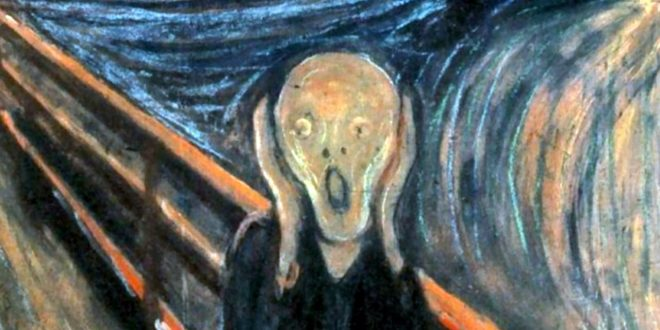
\includegraphics[width=\paperwidth]{munch2.jpg}
%}
%\begin{frame}
%\end{frame}
%}

%\section{Введение в Haskell}


%\defverbatim[colored]{\imageA}{
%\begin{tikzpicture}
%    [%%%%%%%%%%%%%%%%%%%%%%%%%%%%%%
%        box/.style={rectangle,draw=black, ultra thick, minimum size=1cm},
%    ]%%%%%%%%%%%%%%%%%%%%%%%%%%%%%%
%
%\foreach \x/\y in {0/9, 1/\faAmazon,2/13,3/19,4/12,5/8,6/7,7/4,8/21,9/2,10/6,11/11}
%        \node[box] at (\x,0){\y};
%
%\end{tikzpicture}
%}


\begin{frame}{Введение: $\lambda$-исчисление}
  \begin{figure}
    \centering
    \begin{subfigure}[t]{0.45\textwidth}
      \begin{minipage}{0.7\textwidth}
      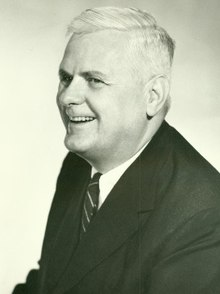
\includegraphics[width=1\textwidth]{220px-Alonzo_Church.jpg}\\
            Alonzo Church (1903–1995)
      \end{minipage}
    \end{subfigure}
    \begin{subfigure}[t]{0.45\textwidth}
      \vspace{-5em}   % TODO: dirty hack!
  Алонзо Чёрч 1935   открыл $\lambda$-исчисление
\vspace{1em}

Аналогичный подход от А.~Тьюринга с его машинами Тьюринга
\vspace{1em}

Это разные подходы для формализации понятия ``алгоритм''
\vspace{1em}

В принципе, могло быть изобретено уже в 1910-х г.г.
\footnotetext{Изображение из \href{https://en.wikipedia.org/wiki/Alonzo\_Church}{Википедии}}

    \end{subfigure}
  \end{figure}

%\thisfloatsetup{heightadjust=all,valign=t}
%\begin{figure}
%  \begin{subfloatrow}
%    \ffigbox[\dimexpr\FBwidth+4cm\relax]
%    {\includegraphics[width=3cm,height=5cm]{example-image-b}}
%    {\caption{Left subfigure}\label{sfig:testa}}%
%    \ffigbox[\FBwidth]
%    {\caption{Right subfigure}\label{sfig:testb}}
%    {\includegraphics[width=3cm,height=2cm]{example-image-a}}
%  \end{subfloatrow}
%\end{figure}

\end{frame}

\begin{frame}{Состояние математики в 1910-х}

    Матан, алгебра, геометрия...\\
    Информатики (computer science) явным образом пока нет, как часть математики\\

    Математическая логика
    \begin{enumerate}
      \item Пытается формализовать интуитивно понятные утверждения
      \item Языки (т.е. синтаксис), чтобы на них можно было правильно сформулировать теоремы
      \item Различные ``семантики'' как интерпретации синтаксиса , потому что формулы могут быть верны и не верны в зависимости от семантики
      \item ``Исчисления'' -- правильные способы доказательств
      \item Теоремы, которые невозможно ни доказать, ни опровергнуть.
    \end{enumerate}
  Начинают задумываться, что такое ``алгоритм'', ``вычисление'' и ``вычислимая функция''

\end{frame}

\begin{frame}{Зачем формализовывать то, что и так понятно?}
\framesubtitle{''Наивная'' теория множеств}
\begin{figure}[t]
  \begin{subfigure}[t]{0.55\textwidth}
    \vspace{-7em}
  Множества можно делить на два типа
  \begin{enumerate}
    \item   набор не является элементом самого себя
    \item Расселовские: набор является элементом самого себя.
  \end{enumerate}
  Рассмотрим $P=\{y: y\notin P\}$ и задумаемся про $P\in P$?
  \begin{itemize}
    \item Если формула верна, то нарушается определение
    \item Если ложна, то не принадлежит, но по определению должна
  \end{itemize}
\footnotetext{Изображение из \href{https://en.wikipedia.org/wiki/Bertrand\_Russell}{Википедии}}

  \end{subfigure}
\hspace{0.05\textwidth}
  \begin{subfigure}[t]{0.35\textwidth}
      \begin{minipage}{0.7\textwidth}
  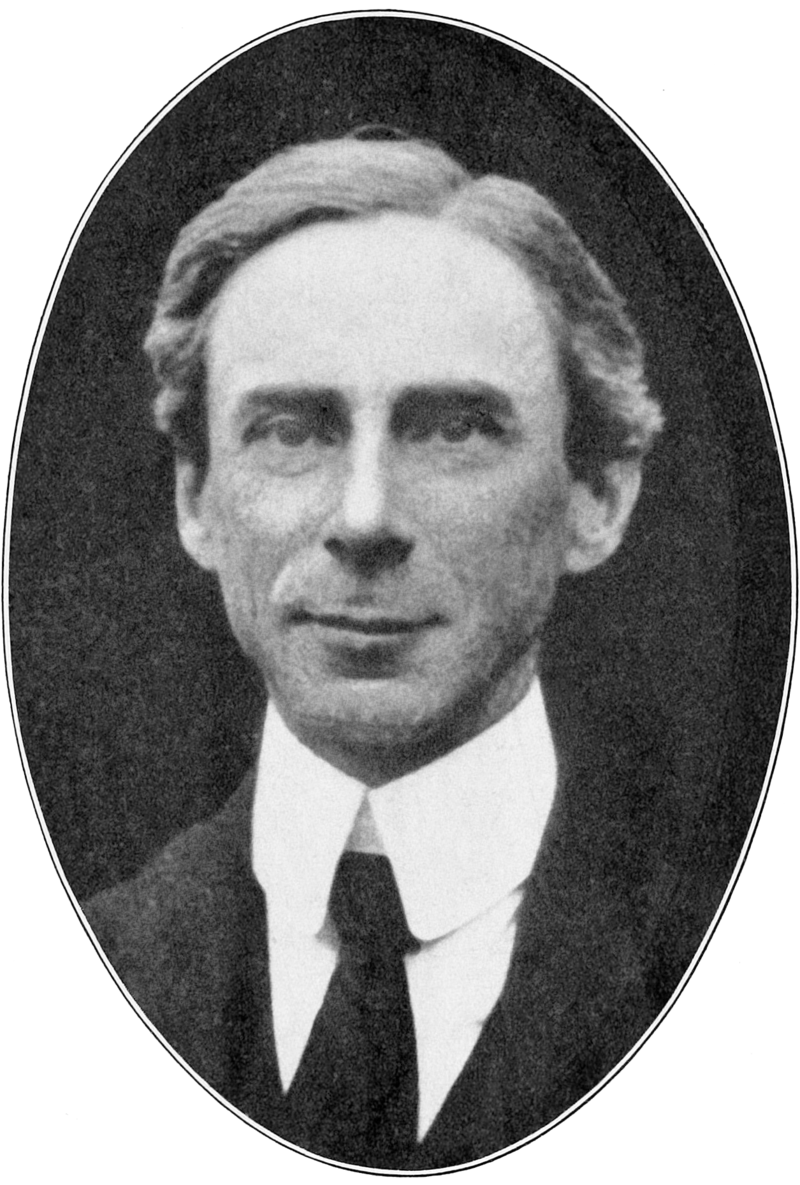
\includegraphics[width=1\textwidth]{800px-Bertrand_Russell_transparent_bg.png}\\
  Bertrand Russell (1872–1970)
\end{minipage}
  \end{subfigure}
\end{figure}
\end{frame}

\begin{frame}{Некоторые известные языки и исчисления из математической логики}
\begin{itemize}
  \item Нулевого порядка (высказываний)
  \item Первого порядка (предикатов)
  \item Высших порядков
  \item Исчисление конструкций (calculus of constructions)
\end{itemize}
\begin{block}{Важное замечание}
  То, что нельзя записать в языке, нельзя использовать в исчислениях/доказательствах
\end{block}
\end{frame}

\begin{frame}{Пример: яызк 0го порядка (высказываний) }
\frametitle{Знакомая вам булева (бинарная) логика}
\begin{figure}[t]
  \begin{subfigure}[t]{0.45\textwidth}
\begin{enumerate}
  \item Логические константы True и False
  \item Логические переменные $x,y,z,\dots$
  \item Бинарные связки $\vee, \wedge, \Rightarrow$ и т.д.
\end{enumerate}
\vspace{2em}
Правила вывода в исчислении, например:
\begin{mathpar}
  \inferrule* [Right=modus ponens]
  { P\Rightarrow Q \\    P  }{Q}
\end{mathpar}
  \end{subfigure}
\hspace{0.05\textwidth}
  \begin{subfigure}[t]{0.46\textwidth}
\begin{theorem}[Язык и исчисление \textbf{``хорошие''}]
  Верную формулу можно доказать за конечное число шагов. Ложную можно опровергнуть.\\

  Т.е. существует алгоритм, который всегда завершается и говорит да/нет.
\end{theorem}
\vspace{2em}
Язык и исчисление \textbf{``плохие''}, потому что не всё можно записать (где кванторы?)
  \end{subfigure}
\end{figure}


\end{frame}


\begin{frame}{Разрешимые и неразрешимые задачи}
  \begin{definition}[Алгоритмически неразрешимая задача]
    Задача, которая имеет ответ ``да'' или ``нет'', но для которое невозможно реализовать алгоритм, который \emph{всегда завершается, и выдает правильный ответ}.
  \end{definition}
  \begin{definition}[Полуразрешимая задача]
    Неразрешимая задача, для которой можно предъявить алгоритм, который либо дает правильный ответ  ``да'', либо не завершается. Полуразрешимые$^{+}$ умеют говорить ``да'', полуразрешимые$^{-}$ --- ``нет''.
  \end{definition}
Как доказывать неразрешимость
\begin{itemize}
  \item Разбирать случаи и искать противоречие в каждом
  \item Сводить каноничную неразрешимую задачу к нашей
\end{itemize}
\end{frame}

\begin{frame}{Язык и исчисление 1-го порядка (предикатов)}
%\framesubtitle{Вы это видели на матане}
\begin{figure}[t]
  \begin{subfigure}[t]{0.5\textwidth}
    Термы:
    \begin{itemize}
      \item Предметные константы: 1.0, 42, $\pi$
      \item Функциональные символы арности  $1\leqslant n$ от термов. Например, $+, \times, f, mod$ и т.д.
    \end{itemize}
    Формулы:
    \begin{itemize}
  \item Логические константы True и False
  \item Логические переменные $x,y,z,\dots$
  \item Бинарные связки $\vee, \wedge, \Rightarrow$ (и т.д.) %(от двух формул)
  \item Предикатные символы (от термов) арности $1\leqslant n$
  \item Кванторы $\forall, \exists$ от имени предметной переменной и формулы
    \end{itemize}
  \end{subfigure}
\hspace{0.05\textwidth}
  \begin{subfigure}[t]{0.4\textwidth}
    \begin{block}{Важно}
      $+, \times, f, mod$ это названия функциональных символов, никто не гарантирует, что  $+$ это сложение чисел
    \end{block}
\vspace{1em}
Пример: \\
$\forall x z\ \exists y (x < y) \vee (y < z)$\\
верно, если $x,y,z \in \mathbb{R}$, \\
неверно, если $x,y,z \in \mathbb{N}$
  \end{subfigure}
\end{figure}
\end{frame}

\begin{frame}{Преимущества и недостатки языка 1го порядка}

  \begin{itemize}
    \item Для некоторых формул из синтаксиса можно понять, что они верны (общезначимы). Для них есть алгоритм, который их докажет за конечное число шагов (см. ``метод британского музея'')
    \item Огромное количество формул верны только в некоторой семантике, для них нельзя предъявить, алгоритм, который завершается и выдает вердикт.\\
    В общем виде проверка формулы на истинность/ложность -- неразрешимая задача
    \item Язык недостаточно богат. Кванторы пробегают только предметные переменные, нельзя выразить ``для любой формулы P, верно...'', например, принцип индукции
    \[
    \forall P.\quad P(0) \Rightarrow (\forall n . P(n) \Rightarrow P(n+1))  \Rightarrow (\forall n . P(n))
    \]
  \end{itemize}
\end{frame}


%\begin{frame}{Недостатки исчисления предикатов}
%Некоторые формулы нельзя записать, а следовательно, пользоваться ими при доказательстве
%
%Например, принцип индукции
%
%
%
%Для этого нужен язык более высокого порядка, чем первого, а там всё ещё хуже с разрешимостью/неразрешимостью
%\end{frame}

\section{Лямбды как апгрейд языка предикатов}

\begin{frame}{Но можно попробовать вывернуться}
\framesubtitle{Введем специальный синтаксис}

\[
\lambda P.\quad phormula(P)
\]
Опишем принцип индукции, и применим его для $P(n)\equiv 0+\dots+n=\frac{n\cdot(n+1)}{2}$
\[
\lambda P.\quad P(0) \Rightarrow \big{(}\forall n . P(n) \Rightarrow P(n+1)\big{)}  \Rightarrow \big{(}\forall n . P(n)\big{)}
\]\pause
\[
\text{применение/подстановка} \mathlarger{\mathlarger{\mathlarger{\mathlarger{\Downarrow  \quad\!\!\!\!\!\!\Uparrow}}}} \text{абстракция}
\]

\begin{equation} \label{eq1}
  \begin{split}
    (0\equiv0) & \Rightarrow (\forall n . (0+\dots+n=\frac{n\cdot(n+1)}{2}) \Rightarrow \Big{(}0+\dots+(n+1)=\frac{(n+1)\cdot(n+2)}{2}\Big{)})  \\
    & \Rightarrow (\forall n . 0+\dots+n=\frac{n\cdot(n+1)}{2})
  \end{split}
\end{equation}
\end{frame}



\begin{frame}{Правила работы с новым языком $\lambda$}
\begin{block}{$\alpha$-эквивалентность}
При выборе новых имен, они не должны случайно перекрыть старые.\\
Предложения языка, отличающиеся только переименованием переменных, считаются ($\alpha$)эквивалентными
\end{block}
Например:  если ни $P$, ни $Q$ не встречаются в $phormula$, то $\lambda P. phormula(P)  \alphaequiv{} \lambda Q. phormula(Q) $

\begin{block}{$\beta$-эквивалентность}
Если у нас встречается $(\lambda P. phormula(P))X$, то мы можем продолжить с этим работать совершив подстановку $X$ вместо $P$ в $phormula$ (записывается как $phormula[P\mapsto X]$), т.е. заменив все свободные вхождения $P$ на $X$ внутри $phormula$.
\end{block}
\end{frame}


\begin{frame}{$\lambda$-исчисление}
Синтаксис
\begin{itemize}
  \item переменные: $x,y,z,\dots$
  \item Абстракция $(\lambda \nu. A)$, где $A$ -- $\lambda$-выражение, а $\nu$ --- произвольное имя переменной
  \item Применение $(AB)$, где $A$ и $B$ --- $\lambda$-выражения
\end{itemize}
\begin{definition}{Редекс}
  --- это $\lambda$-выражение вида $(\lambda \nu. A)B$
\end{definition}
Процесс вычисления --- это процеcc устранения редексов (возможно, не всех) путём подстановок $\lambda$-выражений вместо переменных.
\end{frame}

\begin{frame}{Каррирование%\footnote{}
  }

\begin{figure}[t]
  \begin{subfigure}[t]{0.5\textwidth}
    \vspace{-4em}
В $\lambda$-исчислении функция $n$ аргументов представляются как функция одного аргумента, которые возвращает функцию от $n-1$ аргумента.\\

В мире названо в честь Хаскеля Карри. Впервые появилось в 1924 в работе М.~И.~Шейнфинкеля.\\

\footnotetext{Изображение взято с \href{https://en.wikipedia.org/wiki/Moses\_Sch\%C3\%B6nfinkel}{Википедии}}

  \end{subfigure}
\hspace{1cm}
  \begin{subfigure}[t]{0.3\textwidth}
      \begin{minipage}{1\textwidth}
  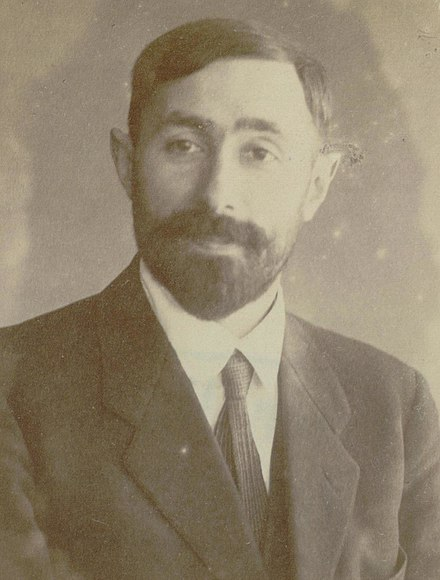
\includegraphics[width=1\textwidth]{440px-Moses_Schonfinkel_1922_(cropped).jpg}\\
  Моисей Исаевич Шейнфинкель (1888 -- 1942)
\end{minipage}
  \end{subfigure}
\end{figure}
\end{frame}


\begin{frame}{Определения алгоритма}
 \begin{theorem}[Тезис Чёрча]
  Используя $\lambda$-исчисление можно реализовать произвольный алгоритм
  \emph{с точностью до представления данных}.
\end{theorem}
\begin{theorem}[Тезис Тьюринга]
Используя машину Тьюринга можно реализовать произвольный алгоритм
\emph{с точностью до представления данных}.
\end{theorem}
Т.е. теперь под алгоритмом понимается только то, что можно записать в формализме.
\end{frame}

\begin{frame}{Как происходят вычисления (редукция) $\lambda$-исчислении?}
  \begin{definition}[Процесс вычислений регламентирует стратегия]
    Ищем редексы $(\lambda x. P)Q$
    \begin{itemize}
      \item Если редексов нет, то вычисление закончилось
      \item Если редексы есть, стратегия регламентирует какой на данном шаге редекс стоит $\beta$-редуцировать
      \item Или же, стратегия может сказать, что все редексы нужно оставить как есть, и выдать ответ.
    \end{itemize}
  \end{definition}
  %Стратегий бывает много разных
  %\begin{enumerate}
  %  \item Строгая стратегия call-by-value .    Для $(\lambda x. P)Q$ вычисляет $Q\cbv Q'$ и потом подставляет $Q'$ вместо $x$ в $P$.
  %  \item Ленивая стратегия call-by-name.   Для $(\lambda x. P)Q$ сразу подставляет $Q$ вместо $x$ в $P$.
  %  \item Обе стратегии оставляют абстракции и переменные как есть
  %\end{enumerate}
\end{frame}

\begin{frame}{Две стратегии: Call-by-value и аппликативная}
  \begin{figure}[t]
    \begin{subfigure}[t]{0.45\textwidth}
            \centering Call-by-value
      \begin{mathpar}
  \inferrule*  [Right=Abs] {\\}
{\lam{x}{e} \cbv \lam{x}{e}}
\end{mathpar}
    \end{subfigure}
    \begin{subfigure}[t]{0.45\textwidth}
      \centering
      Applicative order
      \begin{mathpar}
      \inferrule* [Right=Abs] {e \ao e'}
      {\lam{x}{e} \ao \lam{x}{e'}}
      \end{mathpar}
    \end{subfigure}
  \end{figure}
\hrulefill
\only<1>{
\begin{mathpar}
  \inferrule*  [Right=App-abs]
  { e_1 \arr \lam{x}{e} \\
    e_2 \arr e_2' \\
    [e_2'/x]e \arr e'
  }
  { (e_1 e_2) \arr e'}
\end{mathpar}
\begin{mathpar}
  \inferrule* [Right=Var] {\\}
  {x \arr x}
  \and
  \inferrule*  [Right=App-non-abs]
  { e_1 \arr e' \neq \lam{x}{e} \\
    e_2 \arr e_2'}
  { (e_1 e_2) \arr (e_1' e_2') }
\end{mathpar}
}
\only<2>{
\begin{figure}[t]
  \begin{subfigure}[t]{0.45\textwidth}
\begin{itemize}
\item[\faGood]    Подходит для написания произвольных алгоритмов
\vspace{4em}

\item[\faBad] Не считает под абстракцией, поэтому ответ иногда длиннее, чем хотелось бы
\end{itemize}
  \end{subfigure}
  \begin{subfigure}[t]{0.45\textwidth}
\begin{itemize}
  \item[\faBad] Нет возможности отложить вычисления на потом,т.е. в if-then-else вычисляется и then, и else. Нельзя дождаться ответа от рекурсивных функций
  \item[\faGood] Cчитает под абстракцией, поэтому ответ короче
\end{itemize}
  \end{subfigure}
\end{figure}
}
\end{frame}


\section{Написание алгоритмов с помощью $\lambda$-исчисления}

\begin{frame}{Что нужно для представления алгоритмов?}
  \begin{itemize}
    \item Принимать входные данные
    \item Делать ветвления  в зависимости от входных данных
    \item Совершать некоторое количество однотипных действий в зависимости от входных данных (т.е. должны быть циклы или их аналог -- рекурсия)
    \begin{itemize}
\item       Чтобы понимать, сколько действий уже сделали нужны натуральные числа
    \end{itemize}
  \end{itemize}
\end{frame}

\begin{frame}{Ветвления}
\[
T\equiv\lam{x}{\lam{y}{x}} \equiv fst \qquad \qquad \qquad \qquad
F\equiv \lam{x}{\lam{y}{y}}\equiv snd
\]

\begin{align*}
  ite \quad\equiv &\quad \lambda c. \lambda th. \lambda el. (c\ th\ el)\\
  (ite\ T) \quad\equiv &\quad  \lambda th. \lambda el. (T\ th\ el) \rightsquigarrow th\\
  (ite\ F) \quad\equiv &\quad  \lambda th. \lambda el. (F\ th\ el) \rightsquigarrow el
\end{align*}
\end{frame}

%\section{Представление данных в $\lambda$ исчислении}
\begin{frame}{Представление чисел (Нумералы Чёрча)}

  $ 0 \sim \lam{s}{\lam{x}{x}}$

  $ 1 \sim \lam{s}{\lam{x}{sx}}$

  $ 2 \sim \lam{s}{\lam{x}{s(sx)}}$

  и т.д.
  \vspace{1cm}

  Сложение (один из вариантов): взять два нумерала $m$ и $n$, взять $f$ и $x$, а затем к $x$ применить $n$ раз $f$, а затем к результату применить $m$ раз $f$.

  \[
  add \equiv \lambda m. \lambda n. \lambda f. \lambda x. \app{m\ f\ }{\app{n\ f\ }{x}}
  \]
\end{frame}
\newcommand{\tb}[1]{\textcolor{blue}{#1}}
\newcommand{\tr}[1]{\textcolor{red}{#1}}
\begin{frame}{2+2}
  \begin{align*}
    (\lambda m. \lambda n. \lambda f. \lambda x. \app{m\ f\ }{\app{n\ f\ }{x}}){} 2 2 &\cbv \\
    \textcolor{blue}{(\lambda m. \lambda n. \lambda f. \lambda x. \app{m\ f\ }{\app{n\ f\ }{x}}) {}} \textcolor{red}{2} 2 &\cbv \\
    \textcolor{blue}{( \lambda n. \lambda f. \lambda x. \app{2\ f\ }{\app{n\ f\ }{x}}){}} \textcolor{red}{2} & \cbv \\
    \lambda f. \lambda x. \app{2\ f\ }{\app{2\ f\ }{x}}   &\xarr{\ \ } \\
    \lambda f. \lambda x. \app{\tb{\lam{f}{\lam{x}{f (f x)}}} \ \tr{f}\ }{\app{2\ f\ }{x}} &\ao \\
    \lambda f. \lambda x. \app{\lam{x}{f (f x)} \ \ }{\app{2\ f\ }{x}} &\xarr{\ \ } \\
    \lambda f. \lambda x. \app{\lam{x}{f (f x)} \ \ } {\app{\app{\tb{\lam{f}{\lam{x}{f (f x)}}}\ \tr{f}\ }{x}}} &\ao \\
    \lambda f. \lambda x. \app{\lam{x}{f (f x)}  } {\app{\tb{\lam{x}{f (f x)} } }{\tr{x}}} &\ao \\
    \lambda f. \lambda x. \app{\tb{\lam{x}{f (f x)} } } {\tr{(f (f x))}} &\ao \\
    \lambda f. \lambda x. \lam{x}{f (f (f (f x)))} &
  \end{align*}
\end{frame}


\begin{frame}{2+2}
  \begin{figure}[t]
    \begin{subfigure}[t]{0.50\textwidth}
      \begin{align*}
        (\lambda m. \lambda n. \lambda f. \lambda x. \app{m\ f\ }{\app{n\ f\ }{x}}){} 2 2 &\cbv \\
        \textcolor{blue}{(\lambda m. \lambda n. \lambda f. \lambda x. \app{m\ f\ }{\app{n\ f\ }{x}}) {}} \textcolor{red}{2} 2 &\cbv \\
        \textcolor{blue}{( \lambda n. \lambda f. \lambda x. \app{2\ f\ }{\app{n\ f\ }{x}}){}} \textcolor{red}{2} & \cbv \\
        \lambda f. \lambda x. \app{2\ f\ }{\app{2\ f\ }{x}}   &
      \end{align*}
      Это ответ для $\cbv$.\\

      Давайте посмотрим, что будет, если мы \\
      ответ применим к $g$ и $y$
    \end{subfigure}
    \begin{subfigure}[t]{0.45\textwidth}
      \begin{align*}
        (\lambda f. \lambda x. \app{2\ f\ }{\app{2\ f\ }{x}}) g y  &\cbv \\
        (\lambda x. \app{2\ g\ }{\app{2\ g\ }{x}}) y  &\cbv \\
        \app{2\ g\ }{\app{2\ g\ }{y}}   &\cbv \\
        \app{\tb{\lam{f}{\lam{x}{f (f x)}}} \ \tr{g}\ }{\app{2\ g\ }{y}} &\cbv \\
        \app{\lam{x}{g (g x)} \ \ }{\app{2\ g\ }{y}} &\cbv \\
        \app{\lam{x}{g (g x)} \ \ } {\app{\app{\tb{\lam{f}{\lam{x}{f (f x)}}}\ \tr{g}\ }{x}}} &\cbv \\
        \app{\lam{x}{g (g x)}  } {\app{\tb{\lam{x}{g (g x)} } }{\tr{y}}} &\cbv \\
        \app{\tb{\lam{x}{g (g x)} } } {\tr{(g (g y))}} &\cbv \\
        g (g (g (g y))) &
      \end{align*}
    \end{subfigure}
  \end{figure}
\end{frame}

\begin{frame}{Рекурсия}
Не понятно как вызвать самого себя, так как имен нет.\\

Идея:
\begin{itemize}
  \item записываем фунцию $f$, чтобы она принимала первый аргумент, который будет вызываться вместо рекурсивного вызова
  \item Везде, где надо вызвать эту ``рекурсивную'' функцию, будем писать $Yf$  или $Zf$

  $$
  Y\equiv \lam{f}{\lam{x}{f(x\ x)}\lam{x}{f(x\ x)}}
  $$

  $$
  Z\equiv \lam{f}{\lam{x}{f\lam{v}{\ x\ x\ v}}\lam{x}{f\lam{v}{\ x\ x\ v}}}
  $$
\end{itemize}

\end{frame}


\newcommand{\ite}[3]{\ensuremath{(\text{if } #1\text{ then }#2\text{ else }#3})}}
\begin{frame}{Рекурсия в call-by-value (упрощенно)}
$$
Z\equiv \lam{f}{\lam{x}{f\lam{v}{\ x\ x\ v}}\lam{x}{f\lam{v}{\ x\ x\ v}}}
$$
%Основное свойство
\[
ZR = \lam{x}{R\lam{v}{\ x\ x\ v}} \lam{x}{R\lam{v}{\ x\ x\ v}} \nor
R\big( \lam{x}{R\lam{v}{\ x\ x\ v}}\lam{x}{R\lam{v}{\ x\ x\ v}} \big) =
R(ZR)
\]

\vspace{1em}

Факториал: $fac \equiv (\lambda self.\lambda n . \ite{n<2}{1}{n \cdot self(n-1)})$
\begin{align*}
  Z(\lambda self.\lambda n . \ite{n<2}{1}{n \cdot self(n-1)}) 2 &\cbn \\
  (\lambda n . \ite{n<2}{1}{n \cdot Z\ fac(n-1)}) 2 &\cbn \\
  2 \cdot Y\ fac\ (2-1) &\cbn \\
  2 \cdot (Z(\lambda self.\lambda n . \ite{n<2}{1}{n \cdot self(n-1)})\ 1) &\cbn \\
  2 \cdot \ite{1<2}{1}{n \cdot (Z\ fac\ (1-1))} &\cbn \\
  2 \cdot 1 & \cbn 2
\end{align*}
\end{frame}

%\section{Две стратегии}
\begin{comment}

\begin{frame}{Как происходят вычисления (редукция) $\lambda$-исчислении?}
\begin{definition}[Процесс вычислений регламентирует стратегия]
  Ищем редексы $(\lambda x. P)Q$
\begin{itemize}
  \item Если редексов нет, то вычисление закончилось
  \item Если редексы есть, стратегия регламентирует какой на данном шаге редекс стоит $\beta$редуцировать
  \item Или же, стратегия может сказать, что все редексы нужно оставить как есть, и выдать ответ.
\end{itemize}
\end{definition}
%Стратегий бывает много разных
%\begin{enumerate}
%  \item Строгая стратегия call-by-value .    Для $(\lambda x. P)Q$ вычисляет $Q\cbv Q'$ и потом подставляет $Q'$ вместо $x$ в $P$.
%  \item Ленивая стратегия call-by-name.   Для $(\lambda x. P)Q$ сразу подставляет $Q$ вместо $x$ в $P$.
%  \item Обе стратегии оставляют абстракции и переменные как есть
%\end{enumerate}
\end{frame}

\begin{frame}{Ленивая vs. Строгая}
Пример 1 ($\cbv$ выглядит лучше)\\
$(\lambda x. f x x)((\lambda x. x)A) \cbv (\lambda x. f x x)A \cbv (f A A) \cbv \dots $\\

$(\lambda x. f x x)((\lambda x. x)A) \cbn (\lambda x. f ((\lambda x. x)A) ((\lambda x. x)A))A \cbn \dots $

\vspace{3em}
Пример 2 ($\cbn$ выглядит лучше)\\
$(\lambda x. \lambda y. y)((\lambda x. xx)(\lambda x. xx)) \cbv (\lambda x. \lambda y. y)((\lambda x. xx)(\lambda x. xx)) \cbv \dots \text{зависло}$

$(\lambda x. \lambda y. y)((\lambda x. xx)(\lambda x. xx)) \cbn (\lambda y. y)\quad\text{ответ!}$
\end{frame}
\end{comment}



\begin{comment}


\newcommand{\ite}[3]{\ensuremath{(\text{if } #1\text{ then }#2\text{ else }#3})}}
\begin{frame}{Рекурсия в call-by-name}
$$
Y\equiv \lam{f}{\lam{x}{f(xx)}\lam{x}{f(xx)}}
$$
%Основное свойство
\[
YR = \lam{x}{R(xx)} \lam{x}{R(xx)} \nor
R\big( \lam{x}{R(xx)}\lam{x}{R(xx)} \big) =
R(YR)
\]

\vspace{1em}

Факториал: $fac \equiv (\lambda self.\lambda n . \ite{n<2}{1}{n \cdot self(n-1)})$
\begin{align*}
  Y(\lambda self.\lambda n . \ite{n<2}{1}{n \cdot self(n-1)}) 2 &\cbn \\
  (\lambda n . \ite{n<2}{1}{n \cdot Y\ fac(n-1)}) 2 &\cbn \\
   2 \cdot Y\ fac\ (2-1) &\cbn \\
   2 \cdot (Y(\lambda self.\lambda n . \ite{n<2}{1}{n \cdot self(n-1)})\ 1) &\cbn \\
   2 \cdot \ite{1<2}{1}{n \cdot (Y\ fac\ (1-1))} &\cbn \\
  2 \cdot 1 & \cbn 2
\end{align*}

\end{frame}
\end{comment}


\section{Демка интерпретатора на Си}
\begin{frame}{Дэмка на Си}
  Не забыть показать позднее связывание
\end{frame}

\section*{Вопросы к экзамену (TODO)}
\begin{frame}{Вопросы к экзамену}
\begin{enumerate}
  \item Разрешимые и неразрешимые задачи
  \item $\lambda$-исчисление. $\alpha$ и $\beta$ правила
  \item Нумералы Чёрча. Сложение
  \item Рекурсия и факториал
\end{enumerate}
\end{frame}

%
%\begin{frame}%{Чистые функции}
%\begin{definition}[Неизменяемые структуры данных (immutable data structures)]
%  Которые с течением времени не изменяются \faSmileO
%\end{definition}
%
%\vspace{1em}
%
%\begin{definition}[Устойчивые структуры данных (persistent data structures)]
%Имеют доступ (не уничтожают) предыдущее своё состояние
%\end{definition}
%Почти то же самое, только акцент смещён\vspace{1em}
%
%\begin{remark}
%Так как старые узлы есть, то можно их использовать (share) в новой версии структуры данных
%\end{remark}
%\begin{definition}[Неустойчивые структуры данных называются \textit{эфемерными (ephemeral)}]
%\end{definition}
%\end{frame}



\begin{frame}%[allowframebreaks]
\frametitle<presentation>{Ссылки \& Acknowledgements}
\phantom{\cite*{Harper, HarvardSlides, LitvinovSlides, SESTOFT2001424, Leroy2018}}
\vspace{-1.5em}
\printbibliography
\end{frame}


\begin{frame}{Вопросы к экзамену  }
\begin{enumerate}
	\item \textbf{Определение языка лямбда выражений.} (В вольной формулировке, как минимум из трех пунктов). Редекс, стратегия, подстановка, \textbf{каррирование}, область действия квантора, связанные/свободные вхождения переменных. Формулировка тезиса Чёрча-Тьюринга.
	\item Определение и интуиция за нумералами Чёрча. Определение арифметических операций. \textit{Трассировка сложения и умножения 2 на 2 на листочке.}
	\item Ветвления с помощью λ-исчисления. Идея за комбинатором неподвижной точки. Набросок реализации факториала

\end{enumerate}
\end{frame}
%\appendix



\section{Дополнительные слайды}


\newcommand{\lazy}{\xarr{lazy}}
\newcommand{\strict}{\xarr{strict}}

\begin{frame}{Бывают различные стратегии}
\begin{itemize}
\item Строгие (англ. strict, например, call-by-value) вычисляют аргумент до его подстановки
\item Ленивые (англ. lazy, например, call-by-name)  оставляют вычисление аргумента на потом
\end{itemize}
\vspace{1em}
Классификация по обработке $\lambda$-абстракции
\begin{itemize}
\item Не вычисляют под абстракцией (например, call-by-value $\cbv$)
\item Вычисляют под абстракцией (например, call-by-name $\cbn$)
\end{itemize}
\vspace{2em}

На практике больше любят стратегии, которые эффективно можно посчитать
\end{frame}

\begin{frame}{Ленивая vs. Строгая}
Пример 1 ($\strict$ выглядит лучше)\\
$\lam{x}{f x x}(\tr{(\lambda x. x)}\tb{A}) \strict \tr{(\lambda x. f x x)}\tb{A} \strict (f A\ A) \strict \dots $\\

$\redex{\lam{x}{f x x}}{((\lambda x. x)A)} \lazy f \App{\app{\lam{x}{x}}{A}} {\app{\lam{x}{x}}{A}} \lazy \dots $

\vspace{2em}
Пример 2 ($\lazy$ выглядит лучше)\\
$\lam{x}{\lam{y}{y}}\Redex{\lam{x}{xx}} {\lam{x}{xx}} \strict (\lambda x. \lambda y. y)\Redex{\lam{x}{xx}} {\lam{x}{xx}} \strict \dots \text{зависло}$

$\tr{\lam{x}{\lam{y}{y}}}\tb{\App{\lam{x}{xx}}{\lam{x}{xx}}} \lazy (\lambda y. y)\quad\text{ответ!}$

\vspace{2em}
В обычных языках программирования:
\lstinline[language=c]=(c>0) ? f() : g() =
\end{frame}


\begin{frame}[fragile]{Правила вывода в исчислении}
Пусть дан некоторый язык L, c помощью которого записываются $P_i$ и $C$.\\

\vspace{1em}
Все $(n+1)$-местные правила вывода имеют форму:
\begin{mathpar}
 \inferrule* [leftskip=2em,rightskip=2em,Right={$\qquad$ Название}]
 { P_1\\ ... \\ P_n}
 {C}
\end{mathpar}

\begin{itemize}
  \item $P_i$ --- посылки (premises)
  \item $C_i$ --- заключение (conclusion)
\end{itemize}\vspace{1em}

По смыслу означает <<если и $P_1$, и $P_2$, ..., и $P_n$, то $C$>>

\end{frame}


\begin{frame}{Исчисление}
Состоит из
\begin{itemize}
  \item непустого множества аксиом
  \item множества правил вывода
\end{itemize}
\begin{definition}
Аксиома --- это правило вывода без посылок. Их можно рисовать без черты
\end{definition}
\vspace{2em}
%Формальное определение можно прочитать в книжке Герасимова~\cite{gerasimov}.
\end{frame}


\begin{frame}{Пример исчисления. Дифференциальное исчисление}
Языком L будет язык задания функций (который вообще-то надо формально определять, но не будем)

\begin{mathpar}
  \inferrule* [Right=sin]{\\}
  {sin'(x) = cos(x)}
  \and
  \inferrule* [Right=cos]{\\}
  {cos'(x) = -sin(x)}
  \and
  \inferrule* [Right=var]{\\}
  {x' = 1}
  \and
  \inferrule* [Right=const]{\\}
  {c' = 0, \text{если } c\in N}

\end{mathpar}
\begin{mathpar}
  \inferrule* [Right=mul,leftskip=2em,rightskip=2em]
  {f\ '(x) = u(x) \\ g'(x) = v(x)}
  {((f\cdot g)(x))' = u(x)\cdot g(x) + f(x) \cdot v(x)}
\end{mathpar}
\begin{mathpar}
  \inferrule* [Right=cmps,leftskip=2em,rightskip=2em]
  {f'(x) = u(x) \\ g'(x) = v(x)}
  {(f(g(x)))' = u(g(x)) \cdot v(x)}
\end{mathpar}
\end{frame}


\begin{frame}{Дифференциальное исчисление. Пример вывода}
Вывод обычно рисуется снизу вверх
\begin{mathpar}
\inferrule* []
{ \inferrule* [Right=sin]{ }{\uncover<2- >{sin'(x) =} \uncover<3- >{cos(x)}} \\
  \inferrule* {
    \inferrule* [Right=cos]{ }{\uncover<3- >{cos'(x) =} \uncover<4- >{-sin(x)}} \\
    \inferrule* []
      { \inferrule* [Right=const]{ }{\uncover<4- >{2' = 0}} \\
        \inferrule* [Right=var]{ }{\uncover<4- >{x' = 1}} \\
      }
      {\uncover<3- >{(2\cdot x)' =} \uncover<5- >{0\cdot x + 2\cdot 1} }
  }{\uncover<2- >{cos'(2\cdot x) =} \uncover<6- >{-sin(2\cdot x)\cdot 2} }
}
{(sin(x)\cdot cos(2\cdot x))' = \uncover<7>{cos(x)\cdot cos(2\cdot x) + sin(x)\cdot( -sin(2\cdot x)\cdot 2) }}

\end{mathpar}

На вывод можно смотреть как на \textbf{доказательство} того, что производная действительно посчитана правильно.\\

Результат вывода можно было бы упростить и дальше, но у нас недостаточно правил вывода для этого.
\end{frame}


\begin{frame}{Две стратегии: Call-by-value vs. Full Reduction}
\begin{figure}[ht]
  \begin{subfigure}[t]{.48\textwidth}
     \begin{mathpar}
     \lam{x}{e} \arr \lam{x}{e}
     \and
     \inferrule*  %[Right=App-abs]
     { f \arr \lam{x}{e} \\
       a \arr a_2 \\
       \subst{x}{a_2}{e} \arr r
     }
     { (f a) \arr r}
     \and
     \inferrule* % [Right=App-non-abs]
     { f \arr f_2 \neq \lam{x}{e} \\
       a \arr a_2}
     { (f a) \arr (f_2 a_2) }\\
     v \cbv v\\
    \end{mathpar}
  \end{subfigure}
  \begin{subfigure}[t]{.48\textwidth}
     \begin{mathpar}
     \inferrule* % [Right=App-non-abs]
     { a \arr b }
     { \lam{x}{a} \arr \lam{x}{b}}
      \and
    \inferrule*  %[Right=App-abs]
    { f \arr \lam{x}{e} \\
      a \arr a_2 \\
      \subst{x}{a_2}{e} \arr r
    }
    { (f a) \arr r}
      \and
      \inferrule* % [Right=App-non-abs]
    { f \arr f_2 \neq \lam{x}{e} \\
      a \arr a_2}
    { (f a) \arr (f_2 a_2) }\\
     v \xarr{f\!ull} v
    \end{mathpar}
   \end{subfigure}
\end{figure}


    \begin{figure}[t]
      \begin{subfigure}[t]{0.45\textwidth}
    \begin{itemize}
    \item[\faGood]    Используется в большинстве языков программирования
    \vspace{4em}
    \end{itemize}
      \end{subfigure}
      \begin{subfigure}[t]{0.45\textwidth}
    \begin{itemize}
      \item[\faGood] Cчитает под абстракцией, поэтому короткий ответ
    \end{itemize}
      \end{subfigure}
    \end{figure}
\end{frame}

\begin{frame}{$\lambda$-исчисление. Пример вывода}
Вывод обычно рисуется снизу вверх
\begin{mathpar}
\inferrule* []
{ \inferrule* {
     \inferrule* {
           \inferrule* []{
                \inferrule* []{ }{\uncover<5- >{y \arr y}}
           }{\uncover<4- >{\lam{y}{y} \arr} \uncover<6- >{\lam{y}{y}} } \\
           \inferrule* []{ }{\uncover<4- >{x \arr} \uncover<6- >{x} } \\
           \inferrule* []{ }{\uncover<6- >{\subst{x}{y}{y} \arr x} } \\
        }{\uncover<3- >{ \apppl{\lam{y}{y}}{x} \arr} \uncover<7- >{ x } }
  }{\uncover<2- >{ \lampl{x}{\apppl{\lam{y}{y}}{x}} \arr} \uncover<8- >{ \lam{x}{x} } }\\
  \inferrule* []{ }{\uncover<2- >{a \arr} \uncover<9- >{a}} \\
  \inferrule* []{ }{\uncover<9- >{\subst{a}{x}{x} \arr} \uncover<10- >{a}}
}
{\apppl{\lam{x}{\apppl{\lam{y}{y}}{x}}}{a} \arr \uncover<11- >{a}}
\end{mathpar}


Отличием от дифференциального исчисления будет то, что от результата вывода надо запуститься рекурсивно пока оно не остановится.
Там могло быть также, если бы были правила упрощения (например, $x-x\equiv0$)
%На вывод можно смотреть как на \textbf{доказательство} того, что производная действительно посчитана правильно.\\

%Результат вывода можно было бы упростить и дальше, но у нас недостаточно правил вывода для этого.
\end{frame}


% !TeX root = lambda2023.tex


\defverbatim[colored]{\cast}{
\begin{lstinline}{c}
enum Tag { VAR, ABS, APP };
struct ulc {
  Tag tag;
  union body {
    struct Var { char* name; } Var;
    struct Abs { char* name; ulc* body; } Abs;
    struct App { ulc* f; ulc* arg; } App;
  } body;
};
\end{lstinline}
}

\defverbatim[colored]{\strat}{
\begin{lstlisting}{c}
struct Strategy {
  ulc* (*onVar)(Strategy* self, char* name);
  ulc* (*onApp)(Strategy* self, struct ulc *f, struct ulc *arg);
  ulc* (*onAbs)(Strategy* self, char *name, struct ulc *arg);
};

struct ulc* applyStrategy(Strategy *self, struct ulc *root) {
  switch (root->tag) {
    case VAR: return self->onVar(self, root->body.Var.name);
    case APP: return self->onApp(self, root->body.App.f, root->body.App.arg);
    case ABS: return self->onAbs(self, root->body.Abs.name, root->body.Abs.body);
  }
  assert(false);   return nullptr; // unreachable
}
\end{lstlisting}
}


\defverbatim[colored]{\nostrat}{
\begin{lstinline}
struct ulc *evalVar(Strategy *this, char *name) {
  return var(name);
}
struct ulc *dontReduceUnderAbstraction(Strategy *this, char  *name, ulc *body) {
  return abs(name, body);
}
struct ulc *dontReduceApplication(Strategy *this, ulc* f, ulc* arg) {
  return app(f, arg);
}

struct Strategy NoStrategy = {
  .onvar = evalVar,
  .onApp = dontReduceApplication,
  .onAbs = dontReduceUnderAbstraction,
};
  \end{lstinline}
}

\defverbatim[colored]{\cbvstrat}{
  \begin{lstinline}{c}
struct ulc *evalApplyByValue(Strategy *self, ulc *f, ulc *a1) {
  auto f2 = applyStrategy(self, f);
  switch (f2->tag) {
    case VAR:    case APP:      return app(f2, a1);
    case ABS: {
      auto a2 = applyStrategy(self, a1);
      auto r = subst(a2, f2->body.Abs.name, f2->body.Abs.body);
      return applyStrategy(self, r);
    }
  }
  assert(false); return nullptr; // unreachable
}
struct Strategy CallByValue = {
  .onvar = evalVar,
  .onApp = evalApplyByValue,
  .onAbs = dontReduceUnderAbstraction };
  \end{lstinline}
}

\defverbatim[colored]{\inheritance}{
\begin{lstinline}{c}
struct ulc *evalApplyByValue(Strategy *this, ulc *f, ulc *arg)
struct ulc *evalVar(Strategy *this, char *name);
struct ulc *dontReduceUnderAbstraction(Strategy *this, char *name, ulc *body);
struct ulc *dontReduceApplication(Strategy *this, ulc *f, ulc *arg);

struct Strategy NoStrategy = {
  .onvar = evalVar,
  .onAbs = dontReduceUnderAbstraction,
  .onApp = dontReduceApplication,
};
struct Strategy CallByValue = {
  .onvar = evalVar,
  .onAbs = dontReduceUnderAbstraction
  .onApp = evalApplyByValue,
};
\end{lstinline}
}


\end{document}
